\scanpage{4}
est la condition

e) Le composé de deux\inserted{$\mathcal A_*$} morphismes $X_m\unsure{-|\to}X_n\unsure{-|\to}X_p$ est un $\mathcal A_*$-morphisme.
\margin{Moyennant a) à e)}
\margin{$\operatorname{Hom}_{\mathcal A}(X_m,X_n)\unsure{\hookrightarrow|\longrightarrow}\operatorname{Hom}_{\mathcal A_0\text{-alg}}(\mathcal A_n,\mathcal A_m)$}
\figure{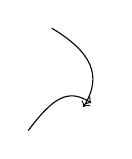
\begin{tikzpicture}[x=1cm,y=1cm]\draw[->] (0,1.3)..controls(.5,1)and(.65,.7)..(.4,.3);\draw[->](-.3,0)..controls(0,.4)and(.2,.55)..(.5,.35);\end{tikzpicture}}
\uline{NB} Moyennant \inserted{b) et} e), la condition a) équivaut au fait que
\[
\left\{\begin{array}{ll}
a_1)&1\in\mathcal A_0\\
a_2)&\text{le morphisme ``addition'' }X_1\times X_1\unsure{-|\to}X_1\text{ est }\mathcal A_*\text{-morph.}\\
a_3)&\rule{2.8cm}{0.3pt}\text{ ``produit'' }X_1\times X_1\unsure{-|\to}X_1\text{ est }\mathcal A_*\text{-morph.}
\end{array}\right.
\]
\uline{NB} Les $\mathcal A_n=k[t_1,\ldots,t_n]$ ou $\mathcal A_n=k[t_1,\ldots,t_n]_{\mathfrak m_n}$ satisfont e)

L'analogue de c) est la condition

f) Si $u:X_n\longrightarrow X_n$ est un $\mathcal A$-morphisme et un isomorphisme, \deleted{alors} i.e. le déterminant \deleted{\unsure{form}} de la matrice jacobienne de $u$ est inversible, alors $u^{-1}$ est un $\mathcal A$-morphisme

Cette condition implique \deleted{\unsure{(et est équivalente à f')}}

f') les $\mathcal A_n$ sont des anneaux henséliens,
\margin{f') implique-t-il f (moyennant a) à e))? il ne semble pas}

[En fait, si f) est satisfait pour un $n$, (f') est satisfait pour $n-1$, i.e. $\mathcal A_{n-1}$ est hensélien]

\deleted{D'ailleurs si $u:X_n\simeq X_n$ est donné par $f_1,\ldots,f_n\in\unsure{B_n|\mathcal A_n}$, alors $u^{-1}$ est donné par $g_1,\ldots,g_n$ appartenant à la clôture hensélienne de $(k[f_1,\ldots,f_n]_{\mathfrak m})$, où $\mathfrak m=k[f_1,\ldots,f_n]$}
\margin{\unsure{vicié?|inutile}}
\figure{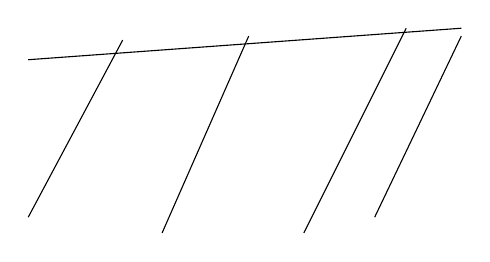
\begin{tikzpicture}[x=1cm,y=1cm]\draw(0,2)--(5.5,2.4);\draw(0,0)--(1.2,2.25);\draw(1.7,-.2)--(2.8,2.3);\draw(3.5,-.2)--(4.8,2.4);\draw(4.4,0)--(5.5,2.3);\end{tikzpicture}}
\uline{NB} Le plus petit $\mathcal A$ satisfaisant a) à d) et f') est formé des
\[
B_n=P\{t_1,\ldots,t_n\}\qquad\text{(clôture hensélienne des }P[t_1,\ldots,t_n]_{\mathfrak m_n}\text{)}
\]
et il satisfait $=$ e) et f).

\deleted{g) Soit $\xi$ un diag de variétés \unsure{for}}

Sous a) b) c) d) e) on définit la catégorie des $\mathcal A$-schémas formels,\inserted{et des Modules dessus (\unsure{finis de t.f.})} et le calcul différentiel dessus (opérateurs différentiels, parties principales,\inserted{\unsure{fibré tangent}} etc.\ $\ldots$)
\margin{(de préférence) \unsure{op. de passage aux produits fibrés} etc.\ $\ldots$}
\margin{3}
